%!TEX program = xelatex

\documentclass[compress]{beamer}
%--------------------------------------------------------------------------
% Common packages
%--------------------------------------------------------------------------

\definecolor{links}{HTML}{663000}
\hypersetup{colorlinks,linkcolor=,urlcolor=links}

\usepackage[english]{babel}
\usepackage{pgfpages} % required for notes on second screen
\usepackage{graphicx}

\usepackage{multicol}

\usepackage{tabularx,ragged2e}
\usepackage{booktabs}

\setlength{\emergencystretch}{3em}  % prevent overfull lines

\usetheme{hri}
\usetikzlibrary{shapes.geometric}
\usetikzlibrary{svg.path, matrix}
\usetikzlibrary{fpu,calc,fit,mindmap,backgrounds,positioning}

% Display the navigation bullet even without subsections
\usepackage{remreset}% tiny package containing just the \@removefromreset command
\makeatletter
\@removefromreset{subsection}{section}
\makeatother
\setcounter{subsection}{1}

\makeatletter
\let\beamer@writeslidentry@miniframeson=\beamer@writeslidentry
\def\beamer@writeslidentry@miniframesoff{%
  \expandafter\beamer@ifempty\expandafter{\beamer@framestartpage}{}% does not happen normally
  {%else
    % removed \addtocontents commands
    \clearpage\beamer@notesactions%
  }
}
\newcommand*{\miniframeson}{\let\beamer@writeslidentry=\beamer@writeslidentry@miniframeson}
\newcommand*{\miniframesoff}{\let\beamer@writeslidentry=\beamer@writeslidentry@miniframesoff}
\makeatother



\newcommand{\source}[2]{{\tiny\it Source: \href{#1}{#2}}}

\usepackage{tikz}
\usetikzlibrary{mindmap,backgrounds,positioning,calc,patterns}

\graphicspath{{figs/}}

\title{Software Architectures for HRI}
\subtitle{~}
\date{}
\author{Séverin Lemaignan}
\institute{{\bf Bristol Robotics Lab}\\University of the West of England}


% for model of anthopomorphism
\newcommand{\IPA}{{$\mathcal{A}_0$~}}
\newcommand{\SLA}{{$\mathcal{A}_\infty$~}}
\newcommand{\sla}{{\mathcal{A}_\infty}}
\newcommand{\AntMax}{{$\mathcal{A}_{max}$~}}
\newcommand{\antMax}{{\mathcal{A}_{max}}}

% for HATP plans
\newcommand{\hatpaction}[3]{#1\\\textsf{\scriptsize #2,}\\\textsf{\scriptsize #3}}
\newcommand{\stmt}[1]{{\footnotesize \tt  #1}}

% for mutual modelling
\newcommand{\Mmodel}[3]{{\mathcal{M}(#1, #2, #3)}}
\newcommand{\model}[3]{{$\mathcal{M}(#1, #2, #3)$}}
\newcommand{\Model}[3]{{$\mathcal{M}^{\circ}(#1, #2, #3)$}}

% typeset logical concept
\newcommand{\concept}[1]{{\scriptsize \texttt{#1}}}

\begin{document}

\miniframesoff

\licenseframe{github.com/severin-lemaignan/lectures-hri-architectures}

\maketitle

\miniframeson

\begin{frame}[plain]{}

    \Large

    \centering
    How hard might it be?

\end{frame}


\begin{frame}{Let's thinker a little...}

    Let's imagine you want to build a robot that {\bf fetches beers from the fridge}
    and bring them back to you whenever you ask. It should {\bf not kill the cat},
    and it should {\bf politely greet your mum} whenever it sees her.

    \begin{columns}
        \begin{column}{0.5\linewidth}

            You have:
            \begin{itemize}
                \item a map with the important landmarks like {\tt fridge}
                \item the following modules:
            \end{itemize}
        \end{column}
        \begin{column}{0.5\linewidth}
            \begin{center}
                \resizebox{\linewidth}{!}{
                    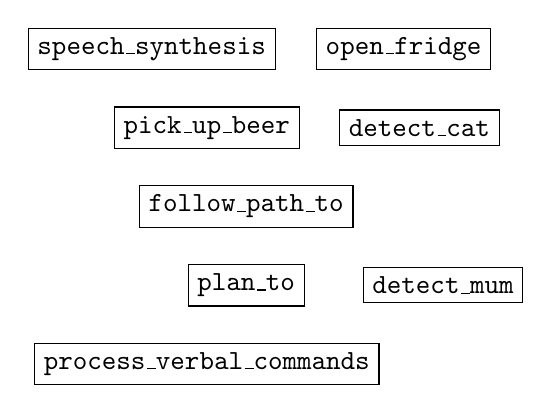
\begin{tikzpicture}[>=latex,every node/.style={draw,font=\tt}]

                        \node at (0.5,2) {follow\_path\_to};
                        \node at (2.5,4) {open\_fridge};
                        \node at (-0.7,4) {speech\_synthesis};
                        \node at (0,0) {process\_verbal\_commands};
                        \node at (3,1) {detect\_mum};
                        \node at (2.7,3) {detect\_cat};
                        \node at (0.5,1) {plan\_to};
                        \node at (0,3) {pick\_up\_beer};
                    \end{tikzpicture}
                }
            \end{center}
        \end{column}
    \end{columns}

    Can you draw a control architecture that achieves just that?
\end{frame}

\begin{frame}{In this lecture}

\begin{itemize}
    \item<+-> Cognitive architectures
    \item<+-> One example of a semantic-aware architecture
\end{itemize}

\end{frame}



%%%%%%%%%%%%%%%%%%%%%%%%%%%%%%%%%%%%%%%%%%%%%%%%%%%%%%%%%%%%%%%%%
%%%%%%%%%%%%%%%%%%%%%%%%%%%%%%%%%%%%%%%%%%%%%%%%%%%%%%%%%%%%%%%%%
%%%%%%%%%%%%%%%%%%%%%%%%%%%%%%%%%%%%%%%%%%%%%%%%%%%%%%%%%%%%%%%%%

\section{Control paradigms}

\begin{frame}{Behavioural (or reactive) control}

    {\bf Behaviours} are small programs that read sensors and control
    actuators. Each behaviour does \textbf{one simple thing}; it typically has
    access to all sensors/actuators.



    \begin{center}
        \only<1>{
        \resizebox{0.5\linewidth}{!}{
            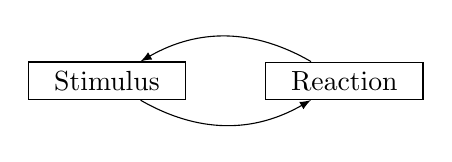
\begin{tikzpicture}[>=latex]
                \node[draw, minimum width=2cm,align=center] at (0,0) (stim) {Stimulus};
                \node[draw, minimum width=2cm,align=center,right=of stim] (reac) {Reaction};
                \path (stim) edge[bend right,->] (reac);
                \path (reac) edge[bend right,->] (stim);
            \end{tikzpicture}
            }
        }
        \only<2>{
        \resizebox{\linewidth}{!}{
            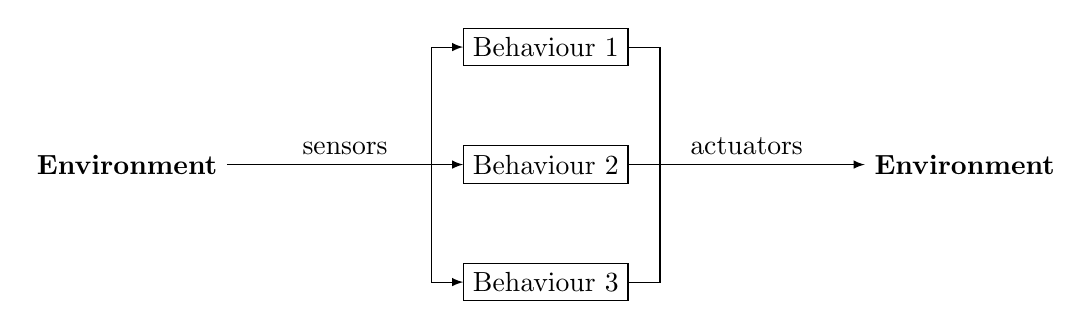
\begin{tikzpicture}[>=latex]
                \node[minimum width=2cm,align=center] at (0,0) (env) {\bf Environment};
                \node[draw, minimum width=2cm,align=center,right=3 of env] (b1) {Behaviour 2};
                \node[draw, minimum width=2cm,align=center,above=of b1] (b2) {Behaviour 1};
                \node[draw, minimum width=2cm,align=center,below=of b1] (b3) {Behaviour 3};
                \node[minimum width=2cm,align=center, right=3 of b1] (env2) {\bf Environment};
                \coordinate[left=0.4 of b1] (a);
                \coordinate[right=0.4 of b1] (b);

                \draw[->] (env)--node[anchor=south, midway]{sensors}(b1);
                \draw[->] (b1)--node[anchor=south, midway]{actuators}(env2);
                \draw[->] (a) |- (b2);
                \draw[->] (a) |- (b3);
                \draw (b) |- (b2);
                \draw (b) |- (b3);
            \end{tikzpicture}
            }

            We only want one behaviour at a time! Need to \textbf{prioritise}:
            behaviours can \emph{override} or \textbf{subsume} less important
            ones.

        }
    \end{center}
    
\end{frame}

\begin{frame}{Extreme case: Braitenberg machines}

    \begin{columns}
        \begin{column}{0.5\linewidth}

            \begin{itemize}
                \item Motion directly controlled by sensors (typically photocells)
                \item Yet the resulting behaviour may appear complex or even intelligent
                \item<1-2> Can you guess the behaviours of vehicles 2a and 2b?
                \item<3-> Complex behaviours emerge (typically with non-linear control functions).
            \end{itemize}

        \end{column}
        \begin{column}{0.5\linewidth}
            \begin{center}
                \includegraphics<1>[width=0.7\linewidth]{Braitenberg_Vehicle_2ab-blind}
                \includegraphics<2->[width=0.7\linewidth]{Braitenberg_Vehicle_2ab}

                \onslide<3>{
                \includegraphics[width=0.7\linewidth]{Braitenberg_Vehicle_4a}
                }

                \source{https://en.wikipedia.org/wiki/Braitenberg_vehicle}{Wikipedia}
            \end{center}
        \end{column}
    \end{columns}

\end{frame}

\begin{frame}{Combining behaviours: example}

    \only<1>{

        Three behaviours:

        \begin{itemize}
            \item {\bf Follow a robot}
                \begin{itemize}
                    \item Sensor: IR communication
                    \item Behaviour: follow another robot
                \end{itemize}
            \item {\bf Avoid obstacle}
                \begin{itemize}
                    \item Sensors: bumpers
                    \item Behaviour: move away from the wall
                \end{itemize}
            \item {\bf Wander}
                \begin{itemize}
                    \item Sensors: encoders
                    \item Behaviour: move forward and turn
                \end{itemize}
        \end{itemize}

        Which behaviour should have the highest priority? the lowest?

        \source{https://www.clear.rice.edu/engi128/Handouts/Lec17-Robotics.pdf}{example borrowed from Rice University ENGI128}
    }
    \only<2->{
        \begin{center}
            \resizebox{0.6\linewidth}{!}{
                \begin{tikzpicture}[>=latex,
                                    every node/.style={draw,minimum width=2cm}]
                    \node at (0,0) (fol) {Follow a robot};
                    \node[below=1 of fol] (wander) {Wander};
                    \node[above=1 of fol] (avoid) {Avoid obstacle};

                    \node[left=1 of fol,anchor=center,rotate=90,minimum width=4cm] (sensors) {Sensors};

                    \draw[thick,->] (sensors) -- (fol);
                    \draw[thick,->] (sensors.south |- wander) -- (wander);
                    \draw[thick,->] (sensors.south |- avoid) -- (avoid);

                    \coordinate[right=1 of fol] (s1);
                    \coordinate[right=2 of wander] (s2);
                    \node[circle,ultra thick,fill=hriSec2Dark,minimum size=5mm] at (s1) (ss1) {\bf S};
                    \node[circle,ultra thick,fill=hriSec2Dark,minimum size=5mm] at (s2) (ss2) {\bf S};

                    \draw[<-] (ss1) -- ($(ss1) + (70:2cm)$) node[draw=none,align=center,above,color=hriSec1Dark] {\small\it subsumption\\ \small\it operator};

                    \draw[thick] (fol) -- (ss1);
                    \draw[thick,->] (avoid) -| (ss1);
                    \draw[thick] (wander) -- (ss2);
                    \draw[thick,->] (ss1) -| (ss2);

                    \node[right=3 of fol,anchor=center,rotate=-90,minimum width=4cm] (act) {Actuators};

                    \draw[thick,->] (ss2) -- (act.south |- ss2);

                    \node[draw=none, above=0.5 of avoid] {\small\emph{highest priority}};
                    \node[draw=none, below=0.5 of wander] {\small\emph{lowest priority}};

                \end{tikzpicture}
            }
        \end{center}

        We combine behaviours by {\bf subsuming} lower-priority behaviours
        whenever a higher-priority behaviour becomes active.

        \onslide<3>{
            $\rightarrow$ \textbf{subsumption architecture}
        }

    }

\end{frame}

\begin{frame}{Behavioural control: strengths/weaknesses}

    {\bf Strengths}

    \begin{itemize}
        \item {\bf Incremental development}
        \item By definition {\bf modular}
        \item Effective to react to events $\rightarrow$ well suited to {\bf
            dynamic environments}
    \end{itemize}

    {\bf Weaknesses}

    \begin{itemize}
        \item {\bf goal-oriented behaviours hard to implement} (``what will my robot do?'')
        \item {\bf importance of the arbiter}: who inhibits (\ie \emph{subsumes}) who might be context-dependent
        \item debugging difficult (need to trace which behaviours are active)
    \end{itemize}


\end{frame}

\begin{frame}{Event-oriented programming: example of Ranger}

    Ranger is a `box on wheels' developed at EPFL

    \begin{center}
        \includegraphics[width=\linewidth]{ranger}
    \end{center}
\end{frame}

\imageframe[color=black]{ranger-side}

\begin{frame}[fragile]{Event-oriented programming}

    {\bf Event-oriented programming} is a possible way of implementing a
    behavioural control paradigm:
    \vspace{1em}

\begin{overprint}
    \onslide<1>
\begin{pythoncode*}{frame=none}

with Ranger() as robot:

    robot.background_blink()
    robot.look_at_touches()

    robot.whenever("dummy", becomes = True)
                                .do(on_dummy)
    robot.whenever("dummy", becomes = False)
                                .do(on_dummy_removed)
    robot.whenever("scale", increase = 0.3).do(on_toy)
    robot.whenever("bumper", becomes = True).do(on_bumper)

    while True:
        time.sleep(0.1)
\end{pythoncode*}

    
    
    \onslide<2>
    \begin{columns}
        \begin{column}{0.45\linewidth}
            \begin{pythoncode*}{frame=none}
def on_dummy(robot):
    robot.look_at_dummy()
    robot.blink()
    sleep = robot.fall_asleep()
    robot.lightbar(RAINBOW).wait()
    sleep.wait()

def on_dummy_removed(robot):
    robot.light_bar(colors.rand())
    robot.wakeup().wait()
    robot.move(0.4, v = 0.8).wait()
    robot.idle().wait()

\end{pythoncode*}
\end{column}
        \begin{column}{0.55\linewidth}
\begin{pythoncode*}{frame=none}
def on_bumper(robot):
    pulse = robot.pulse_row(0)
    while abs(robot.state.v) > 0.01:
        robot.sleep(0.2)
    pulse.cancel()

def on_toy(robot):
    robot.playsound(SOUNDS["toy_in"])
    robot.lightbar(RAINBOW).wait()
\end{pythoncode*}
        \end{column}
    \end{columns}
\end{overprint}
\end{frame}

\imageframe[scale=0.8]{croquignole-expe}

\begin{frame}{}

    \begin{center}
        \includegraphics[width=0.7\linewidth]{ranger-side}

        Note that this is a example of {\bf aimless, purely reactive}, behaviour.
    \end{center}

\end{frame}

%%%%%%%%%%%%%%%%%%%%%%%%%%%%%%%%%%%%%%%%%%%%%%%%%%%%

\begin{frame}{Model-Plan-Act}

    Basic paradigm for {\bf deliberative architectures}.

    \begin{center}
        \resizebox{\linewidth}{!}{
            \begin{tikzpicture}[>=latex,
                                every node/.style={minimum width=4cm}]

                \node[minimum width=2cm] at (0,0) (env) {\bf Environment};
                \coordinate[right=3 of env] (c1);
                \coordinate[right=of c1] (c2);
                \coordinate[right=of c2] (c3);
                \coordinate[right=of c3] (c4);
                \node[draw,fill=hriSec1Comp,align=center,rotate=90] at (c1) (per) {\Large\bf Perceive};
                \node[draw,fill=hriSec2!50,rotate=90,align=center] at (c2) (mod) {\Large\bf Model} edge[<-] (per);
                \node[draw,fill=hriSec3!50,rotate=90,align=center] at (c3) (pla) {\Large\bf Plan} edge[<-] (mod);
                \node[draw,fill=hriSec3Comp!50,rotate=90,align=center] at (c4) (act) {\Large\bf Act} edge[<-] (pla);
                \node[minimum width=2cm,right=3 of c4] (env2) {\bf Environment};

                \draw[->] (env)--node[anchor=south, midway]{sensors}(per);
                \draw[->] (act)--node[anchor=south, midway]{actuators}(env2);
            \end{tikzpicture}
        }
    \end{center}

\end{frame}


\begin{frame}{Task planning}

    \only<1-4>{

    Turn a high-level goal (\emph{bring me a beer!}) into `simple'
    \textbf{primitive} actions.

    A standard approach relies on \textbf{Hierarchical task networks}
    (\textbf{HTN}): uses partial-order contraints to \emph{decompose actions}
    into \emph{primitive operators}.

    \begin{center}
            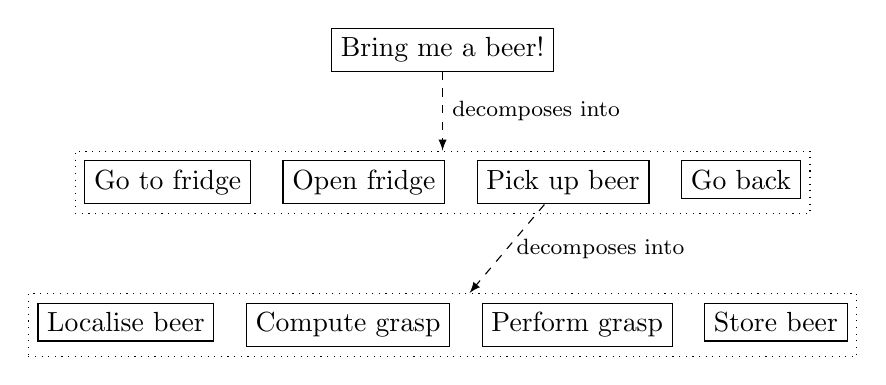
\begin{tikzpicture}[scale=0.3,>=latex,
                                ampersand replacement=\&, % needed when inside beamer frames
                                every node/.style={draw,solid},
                                every edge/.style={solid,ultra thick,<-,draw}]

                \node[draw=none] at (0,0) {}; % just to ensure a constant size for beamer
                \node[draw=none] at (0,-10) {}; % just to ensure a constant size for beamer

                \node<2-> (a1) {Bring me a beer!};

                \matrix<3->[dotted,below=of a1, matrix of nodes,column sep=4mm] (g1){
                        Go to fridge \& Open fridge \& Pick up beer \& Go back \\
                };

                \matrix<4->[dotted,below=of g1, matrix of nodes,column sep=4mm] (g2){
                    Localise beer \& Compute grasp \& Perform grasp \& Store beer \\
                };

                \draw<3->[dashed,->] (a1) -- (g1) node[draw=none,midway,right] {\footnotesize decomposes into};
                \draw<4->[dashed,->] (g1-1-3) -- (g2) node[draw=none,midway,right] {\footnotesize decomposes into};
            \end{tikzpicture}
    \end{center}
    }

    \only<5>{
        What \emph{primitive action} means is system-dependent: what an agent
        considers as primitive can be another agent’s plans.
    }

\end{frame}

\begin{frame}[fragile]{Task planning: actions}

    An action has \textbf{pre-conditions} and \textbf{post-conditions} (or \emph{effects}).

\begin{verbatim}
Action <action name>
{
    preconditions {...};
    effects{...};
    cost{<cost_function_name>};
    duration{<duration_function_name>};
}
\end{verbatim}

\pause

\begin{verbatim}
Action open_fridge
{
    preconditions {facing_fridge AND fridge_door.closed};
    effects {facing_fridge AND fridge_door.open};
}
\end{verbatim}

\end{frame}

\begin{frame}{Example: Shakey the robot}

    Shakey the robot (Stanford, 1968), using the \textbf{STRIPS} planner

    \begin{columns}
        \begin{column}{0.5\linewidth}
                \includegraphics[width=0.8\linewidth]{shakey}
        \end{column}
        \begin{column}{0.5\linewidth}
                \includegraphics[width=\linewidth]{shakey-strips}
        \end{column}
    \end{columns}

\end{frame}

\begin{frame}{Task planning}

    \centering

        \includegraphics[width=0.7\linewidth]{cleantable/manip_run_cam3}

    \resizebox{0.9\linewidth}{!}{%
        \begin{tikzpicture}[
                >=latex,
            robot/.style={fill=hriSec2Comp!50},
            every edge/.style={<-, draw, ultra thick},
            every node/.style={ draw, 
                        thick,  
                        circle, 
                        font=\sf,
                        align=center,
                        node distance=2cm,
                        fill=hriSec3CompDark!50, 
                        minimum size=3cm, 
                        inner sep=0.1cm}]

                    \node<2>[font=\rm\Huge, draw=none, fill=none, rotate=90] at (-3, 0) {Human\\actions};
            \node[font=\rm\Huge, draw=none, fill=none, rotate=90] at (-3, -4.5) {Robot\\actions};

            \coordinate (h1) at (0,0);

            \node<2> at (h1) (hh1) {\bf TAKE\\GREY\_TAPE\\TABLE};
            \node<2>[right=of hh1] (h2) {\bf PUT\\GREY\_TAPE\\BIN1 } edge (hh1);

            \node[robot, below=2.5 of h1] (r1) {\bf TAKE\\BLACK\_TAPE\\TABLE };
            \node[robot, right=of r1] (r2) {\bf PUT\\BLACK\_TAPE\\BIN2 } edge (r1);
            \node[robot, right=of r2] (r3) {\bf TAKE\\BOTTLE\\TABLE } edge (r2);
            \node[robot, right=of r3] (r4) {\bf PUTRV\\BOTTLE\\TABLE} edge (r3);
            \node[robot, right=of r4] (r5) {\bf TAKE\\BOOK\\TABLE } edge (r4);
            \node[robot, right=of r5] (r6) {\bf PUT\\BOOK\\BIN2 } edge (r5);

            \node<2> at (r5 |- h1) (h3) {\bf TAKE\\BOTTLE\\TABLE} edge (h2) edge (r4);
            \node<2>[right=of h3] (h4) {\bf PUT\\BOTTLE\\BIN1} edge (h3);

        \end{tikzpicture}
    }


\end{frame}

\videoframe[0.7]{videos/clean-table.webm}

%%%%%%%%%%%%%%%%%%%%%%%%%%%%%%%%%%%%%%%%%%%%%%%%%%%%%%%%
%{
%\paper{Lemaignan et al. {\bf Artificial Cognition for Social Human-Robot
%     Interaction: An Implementation} Artifical Intelligence, 2016}
\begin{frame}{Full social \& autonomous interaction: one example}

    \begin{center}

     \begin{columns}
         \begin{column}{0.3\linewidth}
                 \includegraphics[height=0.75\paperheight]{clean-table2}
         \end{column}
         \begin{column}{0.7\linewidth}
             \centering
             \resizebox{!}{0.75\paperheight}{%
                 \begin{tikzpicture}[
                         >=latex,
                     every edge/.style={draw, ultra thick, ->},
                     every node/.style={align=center},
                     robot/.style={fill=hriSec2Comp!50},
                     plan/.style={draw,
                      thick,  
                      circle, 
                      font=\sf,
                      align=center,
                      fill=hriSec3CompDark!50, 
                      minimum size=1cm, 
                      inner sep=0.1cm}
                  ]

                     \coordinate (figbottom) at (-0.5, -28.5);


                     \fill[gray!10!white] (4.6,.5) rectangle (figbottom);

                     \path (-0.5,0) edge (figbottom) node[sloped, above left, rotate=90] {\large\bf time};

                     \node at (2,0) (percept) {\bf Perception};
                     \node[below=0.5 of percept.south west, anchor=mid] {camera};
                     \node[below=0.5 of percept.south east, anchor=mid] {3D model};

                     \node[right=4 of percept, minimum width=2.5cm] (kb) {\bf Knowledge};
                     \node[below=0.5 of kb.south west, anchor=mid east] (kbr) {robot};
                     \node[below=0.5 of kb.south east, anchor=mid west] (kbh) {human};
                     \draw[dotted] (kbr) to (figbottom -| kbr);
                     \draw[dotted] (kbh) to (figbottom -| kbh);

                     \fill[gray!10!white] (12,.5) rectangle (17,0 |- figbottom);
                     \node[right=4.5 of kb] (plan) {\bf Plan};
                     \node[below=0.5 of plan.south west, anchor=mid east] (probot) {robot};
                     \node[below=0.5 of plan.south east, anchor=mid west] (phuman) {human};
                     \draw[dotted] (probot) to (figbottom -| probot);
                     \draw[dotted] (phuman) to (figbottom -| phuman);

                     \node[right=5 of plan] (action) {\bf Actions};
                     \node[below=0.5 of action.south west, anchor=mid east] (arobot) {robot};
                     \node[below=0.5 of action.south east, anchor=west] (ahuman) {human\\(monitoring)};
                     \draw[dotted] (arobot) to (figbottom -| arobot);
                     \draw[dotted] (ahuman) to (figbottom -| ahuman);

                     \draw[dashed] (-0.6,-1.2) --(24, -1.2);

                     \node[anchor=east] at (-0.5, -3) (t1) {\Large $t_1$};
                     \node[anchor=east, below=6 of t1] (t2) {\Large $t_2$};
                     \node[anchor=east, below=6 of t2] (t3) {\Large $t_3$};
                     \node[anchor=east, below=4 of t3] (t4) {\Large $t_4$};
                     \node[anchor=east, below=5 of t4] (t5) {\Large $t_5$};

                     %%%%%%%%%%%%%%%%%%%%%%%%%%%%%%%%%%%%%%%%%%%%%%%%%%%%%%%%%%%%%%%%%%%%%%%%%%%%%%%%%%%%%%%%%%%%
                     %%% PERCEPTIONS
                     %%%%%%%%%%%%%%%%%%%%%%%%%%%%%%%%%%%%%%%%%%%%%%%%%%%%%%%%%%%%%%%%%%%%%%%%%%%%%%%%%%%%%%%%%%%%

         \node at (t1 -| percept) (cam1) {\includegraphics[height=2cm]{cleantable/manip_run_cam1.png}};
         \node at (t2 -| percept) (cam2) {\includegraphics[height=2cm]{cleantable/manip_run_cam2.png}};
         \node at (t3 -| percept) (cam3) {\includegraphics[height=2cm]{cleantable/manip_run_cam3.png}};
         \node at (t4 -| percept) (cam4) {\includegraphics[height=2cm]{cleantable/manip_run_cam4.png}};
         \node at (t5 -| percept) (cam5) {\includegraphics[height=2cm]{cleantable/manip_run_cam5.png}};

         %%%%%%%%%%%%%%%%%%%%%%%%%%%%%%%%%%%%%%%%%%%%%%%%%%%%%%%%%%%%%%%%%%%%%%%%%%%%%%%%%%%%%%%%%%%%
         %%% KNOWLEDGE
         %%%%%%%%%%%%%%%%%%%%%%%%%%%%%%%%%%%%%%%%%%%%%%%%%%%%%%%%%%%%%%%%%%%%%%%%%%%%%%%%%%%%%%%%%%%%

         \node[fill=white,align=left] at (cam1 -| kbr) (kb1) {\stmt{TAPE isVisible true}\\
                                                    \stmt{TAPE isReachable true}\\
                                                    \stmt{TAPE isOn TABLE}\\
                                                    \stmt{BIN isVisible true}\\
                                                    \stmt{BIN isReachable false}};

         \node[fill=white,align=left] at (cam1 -| kbh) {\stmt{TAPE isVisible true}\\
                                                    \stmt{TAPE isReachable false}\\
                                                    \stmt{TAPE isOn TABLE}\\
                                                    \stmt{BIN isVisible true}\\
                                                    \stmt{BIN isReachable true}};

         \node[fill=white,align=left] at (cam2 -| kbr) (kb2) {\stmt{ROBOT hasInHand TAPE}};


         \node[fill=white,align=left] at (cam3 -| kbr) {\stmt{TAPE isReachable true}\\
                                        \stmt{TAPE isVisible true} \\
                                        \stmt{TAPE isOn TABLE}};

         \node[fill=white,align=left ] at (cam3 -| kbh) (kb3) {\stmt{TAPE isReachable true}\\
                                         \stmt{TAPE isVisible true}};

         \node[fill=white,align=left] at (cam4 -| kbh) (kb4) {\stmt{HUMAN hasInHand TAPE}};

         \node[fill=white,align=left] at (cam5 -| kbr)  {\stmt{TAPE isIn BIN}};
         \node[fill=white,align=left] at (cam5 -| kbh) (kb5) {\stmt{TAPE isIn BIN}};

         %%%%%%%%%%%%%%%% %%%%%%%%%%%%%%%%%%%%%%%%%%%%%%%%%%%%%%%%%%%%%%%%%%%%%%%%%%%%%%%%%%%%%%%%%%%%
         %%% PLANS
         %%%%%%%%%%%%%%%%%%%%%%%%%%%%%%%%%%%%%%%%%%%%%%%%%%%%%%%%%%%%%%%%%%%%%%%%%%%%%%%%%%%%%%%%%%%%

         \node[fill=gray!10!white,below=1 of plan] (incoming) {\bf \Large Incoming goal \\ \it Clean the table!};

         \node[anchor=north, plan, robot] at (cam1.south -| probot) (pr1) {\bf TAKE\\TAPE\\TABLE};
         \node[anchor=north, plan, robot] at (cam2.south -| probot)  (pr2) {\bf PUTRV\\TAPE\\TABLE} edge[<-] (pr1);
         \node[anchor=north, plan] at (cam3.south -| phuman) (ph1) {\bf TAKE\\TAPE\\TABLE} edge[<-] (pr2);
         \node[anchor=north, plan]  at (cam4.south -| phuman) (ph2) {\bf PUT\\TAPE\\BIN} edge[<-] (ph1);

         \node[fill=gray!10!white,anchor=north] at (cam5.south -| plan) (done) {\bf \Large Goal completed};

         %%%%%%%%%%%%%%%%%%%%%%%%%%%%%%%%%%%%%%%%%%%%%%%%%%%%%%%%%%%%%%%%%%%%%%%%%%%%%%%%%%%%%%%%%%%%
         %%% ACTIONS
         %%%%%%%%%%%%%%%%%%%%%%%%%%%%%%%%%%%%%%%%%%%%%%%%%%%%%%%%%%%%%%%%%%%%%%%%%%%%%%%%%%%%%%%%%%%%

         \only{
             \node[fill=white] at (pr1 -| arobot) (ep1) {\it evaluate pre-conditions};

         \node[below=0.1 of ep1] (mhp1) {%
             \begin{tikzpicture}
                 \node[fill=white] (title) {\bf motion planning};
                 \node[below=0.1 of title.south west, label=below:{\tt PICK\_GOTO}] (mapg) {\includegraphics{cleantable/MHP_ARM_PICK_GOTO}};
                 \node[fill=white,right=of mapg, label=below:{\tt TAKE\_TO\_FREE}] (mattf) {\includegraphics{cleantable/MHP_ARM_TAKE_TO_FREE}} edge[<-] (mapg);
             \end{tikzpicture}
         };
         \node[fill=white,below=0.1 of mhp1] (me1) {\bf motion execution};
         \node[fill=white,below=0.1 of me1] (ae1) {\it assess post-conditions};
     }
     %%%%%%%%%%%%%%%%%%%%%%%%%%%%%%%%%%%%%%%%%%%%%%%%%%%%%%%%%%%%%%%%%%%%%%%%%%%%%%%%%%%%%%%%%%%%%
         \only{
             \node[fill=white] at (pr2 -| arobot) (ep2) {\it evaluate pre-conditions};

         \node[below=0.1 of ep2] (mhp2) {%
             \begin{tikzpicture}
                 \node[fill=white] (title) {\bf motion planning};
                 \node[fill=white,below=0.1 of title, label=below:{\tt ESCAPE}] (maeo) {\includegraphics{cleantable/MHP_ARM_ESCAPE_OBJECT}};
                 \node[left=of maeo, label=below:{\tt PLACE\_FROM\_FREE}] (mapff) {\includegraphics{cleantable/MHP_ARM_PLACE_FROM_FREE}} edge (maeo);
                 \node[fill=white,right=of maeo, label=below:{\tt TO\_FREE}] (maf) {\includegraphics{cleantable/MHP_ARM_FREE}} edge[<-] (maeo);
             \end{tikzpicture}
         };
         \node[fill=white,below=0.1 of mhp2] (me2) {\bf motion execution};
         \node[fill=white,below=0.1 of me2] (ae2) {\it assess post-conditions};
     }
     %%%%%%%%%%%%%%%%%%%%%%%%%%%%%%%%%%%%%%%%%%%%%%%%%%%%%%%%%%%%%%%%%%%%%%%%%%%%%%%%%%%%%%%%%%%%%

         \node[anchor=north] at (ph1 -| ahuman) (wait1) {%
             \begin{tikzpicture}
                 \node[fill=white] (title) {\it wait for pick\\ {\tt TAPE} \it from {\tt TABLE}};
                 \node[below=0.1 of title] {\includegraphics{cleantable/wait_for_pick}};
             \end{tikzpicture}
         };

         \node[anchor=north] at (ph2 -| ahuman) (wait2) {%
             \begin{tikzpicture}
                 \node[fill=white] (title) {\it wait for put\\ {\tt TAPE} \it into {\tt BIN}};
                 \node[below=0.1 of title] {\includegraphics{cleantable/wait_for_throw}};
             \end{tikzpicture}
         };


         %%%%%%%%%%%%%%%%%%%%%%%%%%%%%%%%%%%%%%%%%%%%%%%%%%%%%%%%%%%%%%%%%%%%%%%%%%%%%%%%%%%%%%%%%%%%
         %%% FLOW
         %%%%%%%%%%%%%%%%%%%%%%%%%%%%%%%%%%%%%%%%%%%%%%%%%%%%%%%%%%%%%%%%%%%%%%%%%%%%%%%%%%%%%%%%%%%%
         \draw[dotted, ->, in=45, out=180] (incoming.west) to (kb1);
         \draw[dotted, ->, bend right] (kb1) to (pr1);
         \draw[dotted, ->, bend left] (pr1) to (ep1);
         \draw[dotted, ->, in=45, out=180] (ae1.west) to (kb2);
         \draw[dotted, ->, bend right] (kb2) to (pr2);
         \draw[dotted, ->, bend left] (pr2) to (ep2);
         \draw[dotted, ->, in=45, out=180] (ae2.west) to (kb3);
         \draw[dotted, ->, bend right] (kb3) to (ph1);
         \draw[dotted, ->, bend left] (ph1) to (wait1);
         \draw[dotted, ->, in=-20, out=180] (wait1.west) to (kb4.east);
         \draw[dotted, ->, bend right] (kb4) to (ph2);
         \draw[dotted, ->, bend left] (ph2) to (wait2);
         \draw[dotted, ->, in=20, out=180] (wait2.west) to (kb5);
         \draw[dotted, ->, bend left] (kb5.east) to (done.north);


     \end{tikzpicture}
      }
         \end{column}
     \end{columns}
    \end{center}

\end{frame}
}

\begin{frame}{``Cleaning the table''...}
\centering

\resizebox{!}{0.75\paperheight}{%
\begin{tikzpicture}[
        >=latex,
        every edge/.style={draw, ultra thick, ->},
        every node/.style={align=center},
        robot/.style={fill=hriSec2Comp!50},
        plan/.style={draw,
                     thick,  
                     circle, 
                     font=\sf,
                     align=center,
                     fill=hriSec3CompDark!50, 
                     minimum size=1cm, 
                     inner sep=0.1cm}
        ]

        \coordinate<1> (figbottom) at (-0.5, -28.5);
        \coordinate<2-5> (figbottom) at (-0.5, -10.5);
        \node<2-5> at (0,5) {};
        \node<2-5> at ($(figbottom) + (0,-5)$) {};


        \fill[gray!10!white] (4.6,.5) rectangle (figbottom);

        \path (-0.5,0) edge (figbottom) node[sloped, above left, rotate=90] {\large\bf time};

        \node at (2,0) (percept) {\bf Perception};
            \node[below=0.5 of percept.south west, anchor=mid] {camera};
            \node[below=0.5 of percept.south east, anchor=mid] {3D model};

        \node[right=4 of percept, minimum width=2.5cm] (kb) {\bf Knowledge};
            \node[below=0.5 of kb.south west, anchor=mid east] (kbr) {robot};
            \node[below=0.5 of kb.south east, anchor=mid west] (kbh) {human};
            \draw[dotted] (kbr) to (figbottom -| kbr);
            \draw[dotted] (kbh) to (figbottom -| kbh);

        \fill[gray!10!white] (12,.5) rectangle (17,0 |- figbottom);
        \node[right=4.5 of kb] (plan) {\bf Plan};
            \node[below=0.5 of plan.south west, anchor=mid east] (probot) {robot};
            \node[below=0.5 of plan.south east, anchor=mid west] (phuman) {human};
            \draw[dotted] (probot) to (figbottom -| probot);
            \draw[dotted] (phuman) to (figbottom -| phuman);

        \node[right=5 of plan] (action) {\bf Actions};
            \node[below=0.5 of action.south west, anchor=mid east] (arobot) {robot};
            \node[below=0.5 of action.south east, anchor=west] (ahuman) {human\\(monitoring)};
            \draw[dotted] (arobot) to (figbottom -| arobot);
            \draw[dotted] (ahuman) to (figbottom -| ahuman);

        \draw[dashed] (-0.6,-1.2) --(24, -1.2);

        \node<1,2>[anchor=east] at (-0.5, -3) (t1) {\Large $t_1$};
        \node<1,2>[anchor=east, below=6 of t1] (t2) {\Large $t_2$};
        \node<3>[anchor=east] at (-0.5, -3) (t2) {\Large $t_2$};
        \node<1,3>[anchor=east, below=6 of t2] (t3) {\Large $t_3$};
        \node<4>[anchor=east] at (-0.5, -3) (t3) {\Large $t_3$};
        \node<1,4>[anchor=east, below=4 of t3] (t4) {\Large $t_4$};
        \node<5>[anchor=east] at (-0.5, -3) (t4) {\Large $t_4$};
        \node<1,5>[anchor=east, below=5 of t4] (t5) {\Large $t_5$};

        %%%%%%%%%%%%%%%%%%%%%%%%%%%%%%%%%%%%%%%%%%%%%%%%%%%%%%%%%%%%%%%%%%%%%%%%%%%%%%%%%%%%%%%%%%%%
        %%% PERCEPTIONS
        %%%%%%%%%%%%%%%%%%%%%%%%%%%%%%%%%%%%%%%%%%%%%%%%%%%%%%%%%%%%%%%%%%%%%%%%%%%%%%%%%%%%%%%%%%%%

        \node<1,2> at (t1 -| percept) (cam1) {\includegraphics[height=2cm]{cleantable/manip_run_cam1.png}};
        \node<1,3> at (t2 -| percept) (cam2) {\includegraphics[height=2cm]{cleantable/manip_run_cam2.png}};
        \node<1,4> at (t3 -| percept) (cam3) {\includegraphics[height=2cm]{cleantable/manip_run_cam3.png}};
        \node<1,5> at (t4 -| percept) (cam4) {\includegraphics[height=2cm]{cleantable/manip_run_cam4.png}};
        \node<1,5> at (t5 -| percept) (cam5) {\includegraphics[height=2cm]{cleantable/manip_run_cam5.png}};

        %%%%%%%%%%%%%%%%%%%%%%%%%%%%%%%%%%%%%%%%%%%%%%%%%%%%%%%%%%%%%%%%%%%%%%%%%%%%%%%%%%%%%%%%%%%%
        %%% KNOWLEDGE
        %%%%%%%%%%%%%%%%%%%%%%%%%%%%%%%%%%%%%%%%%%%%%%%%%%%%%%%%%%%%%%%%%%%%%%%%%%%%%%%%%%%%%%%%%%%%

        \node<1,2>[fill=white,align=left] at (cam1 -| kbr) (kb1) {\stmt{TAPE isVisible true}\\
                                                        \stmt{TAPE isReachable true}\\
                                                        \stmt{TAPE isOn TABLE}\\
                                                        \stmt{BIN isVisible true}\\
                                                        \stmt{BIN isReachable false}};

        \node<1,2>[fill=white,align=left] at (cam1 -| kbh) {\stmt{TAPE isVisible true}\\
                                                        \stmt{TAPE isReachable false}\\
                                                        \stmt{TAPE isOn TABLE}\\
                                                        \stmt{BIN isVisible true}\\
                                                        \stmt{BIN isReachable true}};

        \node<1,3>[fill=white,align=left] at (cam2 -| kbr) (kb2) {\stmt{ROBOT hasInHand TAPE}};


        \node<1,4>[fill=white,align=left] at (cam3 -| kbr) {\stmt{TAPE isReachable true}\\
                                            \stmt{TAPE isVisible true} \\
                                            \stmt{TAPE isOn TABLE}};

        \node<1,4>[fill=white,align=left ] at (cam3 -| kbh) (kb3) {\stmt{TAPE isReachable true}\\
                                             \stmt{TAPE isVisible true}};

        \node<1,5>[fill=white,align=left] at (cam4 -| kbh) (kb4) {\stmt{HUMAN hasInHand TAPE}};

        \node<1,5>[fill=white,align=left] at (cam5 -| kbr)  {\stmt{TAPE isIn BIN}};
        \node<1,5>[fill=white,align=left] at (cam5 -| kbh) (kb5) {\stmt{TAPE isIn BIN}};

        %%%%%%%%%%%%%%%% %%%%%%%%%%%%%%%%%%%%%%%%%%%%%%%%%%%%%%%%%%%%%%%%%%%%%%%%%%%%%%%%%%%%%%%%%%%%
        %%% PLANS
        %%%%%%%%%%%%%%%%%%%%%%%%%%%%%%%%%%%%%%%%%%%%%%%%%%%%%%%%%%%%%%%%%%%%%%%%%%%%%%%%%%%%%%%%%%%%

        \node<1,2>[fill=gray!10!white,below=1 of plan] (incoming) {\bf \Large Incoming goal \\ \it Clean the table!};

        \node<1,2>[anchor=north, plan, robot] at (cam1.south -| probot) (pr1) {\bf TAKE\\TAPE\\TABLE};
        \node<1,3>[anchor=north, plan, robot] at (cam2.south -| probot)  (pr2) {\bf PUTRV\\TAPE\\TABLE} edge[<-] (pr1);
        \node<1,4>[anchor=north, plan] at (cam3.south -| phuman) (ph1) {\bf TAKE\\TAPE\\TABLE} edge[<-] (pr2);
        \node<1,5>[anchor=north, plan]  at (cam4.south -| phuman) (ph2) {\bf PUT\\TAPE\\BIN} edge[<-] (ph1);

        \node<1,5>[fill=gray!10!white,anchor=north] at (cam5.south -| plan) (done) {\bf \Large Goal completed};

        %%%%%%%%%%%%%%%%%%%%%%%%%%%%%%%%%%%%%%%%%%%%%%%%%%%%%%%%%%%%%%%%%%%%%%%%%%%%%%%%%%%%%%%%%%%%
        %%% ACTIONS
        %%%%%%%%%%%%%%%%%%%%%%%%%%%%%%%%%%%%%%%%%%%%%%%%%%%%%%%%%%%%%%%%%%%%%%%%%%%%%%%%%%%%%%%%%%%%

        \only<1,2>{
        \node[fill=white] at (pr1 -| arobot) (ep1) {\it evaluate pre-conditions};

        \node[below=0.1 of ep1] (mhp1) {%
            \begin{tikzpicture}
                \node[fill=white] (title) {\bf motion planning};
                \node[below=0.1 of title.south west, label=below:{\tt PICK\_GOTO}] (mapg) {\includegraphics{cleantable/MHP_ARM_PICK_GOTO}};
                \node[fill=white,right=of mapg, label=below:{\tt TAKE\_TO\_FREE}] (mattf) {\includegraphics{cleantable/MHP_ARM_TAKE_TO_FREE}} edge[<-] (mapg);
            \end{tikzpicture}
        };
        \node[fill=white,below=0.1 of mhp1] (me1) {\bf motion execution};
        \node[fill=white,below=0.1 of me1] (ae1) {\it assess post-conditions};
        }
        %%%%%%%%%%%%%%%%%%%%%%%%%%%%%%%%%%%%%%%%%%%%%%%%%%%%%%%%%%%%%%%%%%%%%%%%%%%%%%%%%%%%%%%%%%%%%
        \only<1,3>{
        \node[fill=white] at (pr2 -| arobot) (ep2) {\it evaluate pre-conditions};

        \node[below=0.1 of ep2] (mhp2) {%
            \begin{tikzpicture}
                \node[fill=white] (title) {\bf motion planning};
                \node[fill=white,below=0.1 of title, label=below:{\tt ESCAPE}] (maeo) {\includegraphics{cleantable/MHP_ARM_ESCAPE_OBJECT}};
                \node[left=of maeo, label=below:{\tt PLACE\_FROM\_FREE}] (mapff) {\includegraphics{cleantable/MHP_ARM_PLACE_FROM_FREE}} edge (maeo);
                \node[fill=white,right=of maeo, label=below:{\tt TO\_FREE}] (maf) {\includegraphics{cleantable/MHP_ARM_FREE}} edge[<-] (maeo);
            \end{tikzpicture}
        };
        \node[fill=white,below=0.1 of mhp2] (me2) {\bf motion execution};
        \node[fill=white,below=0.1 of me2] (ae2) {\it assess post-conditions};
        }
        %%%%%%%%%%%%%%%%%%%%%%%%%%%%%%%%%%%%%%%%%%%%%%%%%%%%%%%%%%%%%%%%%%%%%%%%%%%%%%%%%%%%%%%%%%%%%

        \node<1,4>[anchor=north] at (ph1 -| ahuman) (wait1) {%
            \begin{tikzpicture}
                \node[fill=white] (title) {\it wait for pick\\ {\tt TAPE} \it from {\tt TABLE}};
                \node[below=0.1 of title] {\includegraphics{cleantable/wait_for_pick}};
            \end{tikzpicture}
        };

        \node<1,5>[anchor=north] at (ph2 -| ahuman) (wait2) {%
            \begin{tikzpicture}
                \node[fill=white] (title) {\it wait for put\\ {\tt TAPE} \it into {\tt BIN}};
                \node[below=0.1 of title] {\includegraphics{cleantable/wait_for_throw}};
            \end{tikzpicture}
        };


        %%%%%%%%%%%%%%%%%%%%%%%%%%%%%%%%%%%%%%%%%%%%%%%%%%%%%%%%%%%%%%%%%%%%%%%%%%%%%%%%%%%%%%%%%%%%
        %%% FLOW
        %%%%%%%%%%%%%%%%%%%%%%%%%%%%%%%%%%%%%%%%%%%%%%%%%%%%%%%%%%%%%%%%%%%%%%%%%%%%%%%%%%%%%%%%%%%%
        \draw<1,2>[dotted, ->, in=45, out=180] (incoming.west) to (kb1);
        \draw<1,2>[dotted, ->, bend right] (kb1) to (pr1);
        \draw<1,2>[dotted, ->, bend left] (pr1) to (ep1);
        \draw<1,2>[dotted, ->, in=45, out=180] (ae1.west) to (kb2);
        \draw<1,3>[dotted, ->, bend right] (kb2) to (pr2);
        \draw<1,3>[dotted, ->, bend left] (pr2) to (ep2);
        \draw<1>[dotted, ->, in=45, out=180] (ae2.west) to (kb3);
        \draw<1,4>[dotted, ->, bend right] (kb3) to (ph1);
        \draw<1,4>[dotted, ->, bend left] (ph1) to (wait1);
        \draw<1>[dotted, ->, in=-20, out=180] (wait1.west) to (kb4.east);
        \draw<1,5>[dotted, ->, bend right] (kb4) to (ph2);
        \draw<1,5>[dotted, ->, bend left] (ph2) to (wait2);
        \draw<1,5>[dotted, ->, in=20, out=180] (wait2.west) to (kb5);
        \draw<1,5>[dotted, ->, bend left] (kb5.east) to (done.north);


 \end{tikzpicture}
 }
\end{frame}





%%%%%%%%%%%%%%%%%%%%%%%%%%%%%%%%%%%%%%%%%%%%%%%%%%%%%%%%%%%%%%%%%%%
%%%%%%%%%%%%%%%%%%%%%%%%%%%%%%%%%%%%%%%%%%%%%%%%%%%%%%%%%%%%%%%%%%%
%%%%%%%%%%%%%%%%%%%%%%%%%%%%%%%%%%%%%%%%%%%%%%%%%%%%%%%%%%%%%%%%%%%

\section{Integrating into an architecture}

\begin{frame}[label=ctrlstrategies]{Control strategies}

    {\bf Behavioural} or reactive

    \begin{itemize}
        \item \emph{bottom-up} approach
        \item lots of independent modules executing concurrently,
            monitoring sensor values, triggering actions and possibly inhibiting each-others
        \item hard to organize into complex behaviours; gets messy quickly
    \end{itemize}

    \pause

    {\bf Hierarchical}: classic model/plan/act

    \begin{itemize}
        \item \emph{top-down} approach
        \item starts with high-level goals, decompose into sub-tasks
        \item not very agile
    \end{itemize}

    \pause

    {\bf Hybrid approaches?}

    \begin{itemize}
        \item Deliberative at high level, reactive at low level
    \end{itemize}

\end{frame}

\begin{frame}{Levels of control}
    Control problems are usually split into three levels:

    \begin{itemize}
        \item<1-> \textbf{Low-level control}
            \begin{itemize}
                \item Example: where to place a leg as robot takes its next step
                \item Generally, continuous-valued problems
                \item Short time scale (under a second); high frequency loop
            \end{itemize}
        \item<2-> \textbf{Intermediate level control}
            \begin{itemize}
                \item Navigating to a destination, or picking up an object
                    $\rightarrow$ \emph{capabilities}
                \item Continuous or discrete valued problems
                \item Time scale of a few seconds
            \end{itemize}
        \item<3-> \textbf{High level control}
            \begin{itemize}
                \item What is the plan for moving these boxes out of the room?
                \item Discrete problems, long time scale (minutes)
            \end{itemize}
    \end{itemize}

    \source{https://www.cs.cmu.edu/afs/cs/academic/class/15494-s11/lectures/architectures.pdf}{CMU lecture on Cognitive Robotics}
\end{frame}

\begin{frame}{Layered Architectures}
    \begin{center}
        %\resizebox{\linewidth}{!}{
            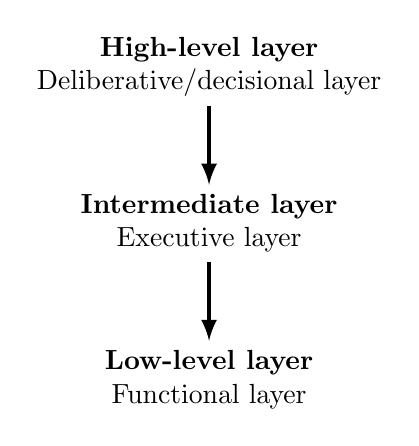
\begin{tikzpicture}[>=latex,every node/.style={minimum width=4cm,align=center}]
                
                \node (low) {\bf Low-level layer\\Functional layer};
                \node[above=of low] (mid) {\bf Intermediate layer\\Executive layer} edge[ultra thick,->] (low);
                \node[above=of mid] (hig) {\bf High-level layer\\Deliberative/decisional layer} edge[ultra thick,->] (mid);

            \end{tikzpicture}
        %}
    \end{center}

    Each layer has different time constraints (from real-time to possibly `slow'); they typically use different control paradigms
\end{frame}


\begin{frame}{Deliberative architecture for interaction}

    One example: the LAAS deliberative architecture for interaction

    \begin{center}
        \includegraphics[width=0.8\linewidth]{clean-table}
    \end{center}
\end{frame}


{
    \paper{Lemaignan et al., {\bf Artificial Cognition for Social Human-Robot
    Interaction: An Implementation}, Artifical Intelligence, 2017}
\begin{frame}<1-6>[label=archi]{A symbolic control architecture}
    \begin{figure}
        \centering

        \resizebox{0.9\paperwidth}{!}{%

            
            \newcommand{\dimming}{50}

            \tikzset{subpart/.style={draw, font=\scriptsize, fill opacity=0.5, text opacity=1, fill=white!50}}

            \begin{tikzpicture}[
                    >=latex,
                    every edge/.style={draw, very thick},
                    skill/.style={draw, rounded corners, align=center, inner sep=5pt, fill=black!20},
    stmt/.style={align=center, font=\bf},
                label/.style={midway, align=center, font=\scriptsize, fill=white}]


                %%% Separation between deliberative layer and sensori-motor layer
                \draw[dotted, thick] (-8,-5) -- (12, -5);

                %%% SPARK
                \uncover<2->{
                    \node at (4,-3.5)[skill, fill=hriSec3!\dimming] (spark) {%
                    \begin{tikzpicture}
          \node at (0,0) (geom) {{\bf Situation Assessment} -- geometric \& temporal reasoning};
                        \node [subpart, below=0.2 of geom.south west, anchor=north west] (world-update) {Sensors fusion};
                        \node [subpart, right=0.2 of world-update] (geom-model) {Geometric model of the environment};
                        \node [subpart, right=0.2 of geom-model] (fact-prod) {Symbolic facts production};
                    \end{tikzpicture}
                };
                }

                %%% LOWLEVEL
                \node [skill, below=0.7 of spark,fill=gray!\dimming] (lowlevel) {%
                    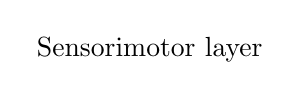
\begin{tikzpicture}
                        \node at (0,0) (sensori) {Sensorimotor layer};
                        %\node [subpart, below=0.2 of sensori.south west, anchor=north west, align=left] (perception) {{\bf Perception} \\ 2D markers, RGB-D, motion capture};
                        %\node [subpart, align=right, right=0.2 of perception] {{\bf Actuation} \\ Head's pan-tilt unit, grippers, arms, wheels};
                    \end{tikzpicture}
                };

                \uncover<2->{
                \path (lowlevel) edge [->] (spark);
                }

                %%% ORO
                \uncover<3->{
                \node at (0,0)[skill, ultra thick, fill=hriSec2Dark!\dimming] (oro) {{\bf Memory} knowledge base(s)\\ \footnotesize typically a symbolic blackboard};
                \path (spark.100) edge [->, bend right] node[label](symfact) {symbolic \\ facts} (oro);
                }

                %%% HATP
                \uncover<5->{
                \node at (-6, 2.5)[skill, fill=hriSec1!\dimming] (hatp) {{\bf Task planner}\\ \footnotesize ideally human-aware};
                \path (hatp) edge [<->, bend right] node[label](domain) {world model and \\ agents beliefs} (oro.170);
                }

                %%% DIALOGS
                \uncover<4->{
                \node at (-6, -3) [skill, fill=hriSec3Dark!\dimming] (dialogs) {{\bf Multi-modal communication}\\NLP, back-channel,...};
                \path (dialogs) edge [<->, bend left] node[label](nlp) {natural language \\ grounding} (oro.190);
                }
                %%% SHARY
                \uncover<5->{
                \node at (4,4.5)[skill, fill=hriSec1Comp!\dimming] (shary) {%
                    \begin{tikzpicture}
                        \node at (0,0) (exec) {\bf Execution Controller};
                        \node [subpart, below=0.2 of exec.south west, anchor=north west] (plans) {Goal \& Plans \\ management};
                        \node [subpart, right=0.2 of plans] (sit-asses) {Situation assessment \\ and context management};
                        \node [subpart, right=0.2 of sit-asses] {Action instantiation, \\ execution and monitoring};
                    \end{tikzpicture}
                };
                \path (shary) edge [<->, bend left] node[label](evts) {events, \\ world model and \\ agents beliefs} (oro);
                \path (shary) edge [<->, bend left, looseness=0.8] node[label] {action monitoring \\ and management of \\ position hypotheses} (spark);
                \path (shary.west) edge [<->, bend right] node[label] {shared \\ plans} (hatp);
                }
                %%% MHP
                \uncover<6->{
                \node at (9,0)[skill, fill=hriSec3CompDark!\dimming] (mhp) {Motion and manipulation \\ planning};
                \path (shary.340) edge [<->, bend left] node[label] {motion plan \\ requests} (mhp);
                \path (spark.5) edge [->, bend right] node[label] {environment\\model} (mhp);
                \path (lowlevel.east) edge [<-, bend right=60, looseness=1.3] node[label] {atomic\\actions} (mhp.south east);
                }



  \only<7>{
      \fill[fill opacity=.7,white] (current bounding box.north west) rectangle (current bounding box.south east);
      \node[stmt] at (symfact) {isOn(bottle, table)\\lookAt(human1, bottle)};
      \node[stmt] at (nlp) {lookAt(human1, ?obj)\\desires(human1, PickUp, bottle)};
      \node[stmt] at (domain) {isAvailable(?gripper) $\wedge$ isA(?gripper, Gripper)\\isOn(bottle, ?obj)};
      \node[stmt] at (evts) {isA(action23425, PickUp) $\wedge$ currentlyPerforming(action23425)};
  }
            \end{tikzpicture}
        }
    \end{figure}


\end{frame}
%}


%\videoframe[0.56]{videos/dialogs.webm}
\videoframe[0.56]{videos/dialogs.webm?autostart}


%%%%%%%%%%%%%%%%%%%%%%%%%%%%%%%%%%%%%%%%%%%%%%%%%%%%%%%%%%%%%%%%%
%%%%%%%%%%%%%%%%%%%%%%%%%%%%%%%%%%%%%%%%%%%%%%%%%%%%%%%%%%%%%%%%%
%%%%%%%%%%%%%%%%%%%%%%%%%%%%%%%%%%%%%%%%%%%%%%%%%%%%%%%%%%%%%%%%%

\section{Cognitive Architectures}

\begin{frame}{Cognitive Architecture?}
\centering
        \resizebox{!}{0.7\paperheight}{%
            \begin{tikzpicture}[
                    >=latex,
                every edge/.style={<-, draw, very thick}]
        

            \path[small mindmap, 
                level 1 concept/.append style={sibling angle=360/5}, 
                level 2 concept/.append style={sibling angle=120}, 
            concept color=hriWarmGreyLight,text=hriWarmGreyDark]
            node[concept] {Cognition}
            [clockwise from=-30]
            child[concept color=hriSec1,text=white] { node[concept] (percept) {Perception}
                [clockwise from=40]
                child[concept color=hriSec2Dark,text=white] { node[concept]{Attention} }
                child[concept color=hriSec2CompDark,text=white] { node[concept] (dialog) {Communication} }
            }
            child[concept color=hriSec2Comp,text=white] { node[concept] (krr) {Knowledge Representation} 
                [clockwise from=-30]
                child[concept color=hriSec1CompDark,text=white] { node[concept] (memory) {Memory} }
                child[concept color=hriSec3CompDark,text=white] { node[concept] (tom) {Theory of Mind} }
            }
            child[concept color=hriSec2,text=white] { node[concept] (action) {Action Execution} 
                [counterclockwise from=110]
                child[concept color=hriSec3,text=white] { node[concept] (plan) {Task Planning} }
                child[concept color=hriSec2CompDark,text=white] { node[concept] (comm) {Communication} }
            }
            child[concept color=hriSec3Comp,text=white] { node[concept] (learning) {Learning} 
                [counterclockwise from=130]
                child[concept color=hriSec1CompDark,text=white] { node[concept] (adapt) {Adaptation} }
            }
            child[concept color=hriSec3CompDark,text=white] { node[concept] (reason) {Reasoning} 
                [clockwise from=110]
                child[concept color=hriSec3Dark,text=white] { node[concept] {Problem solving} }
                child[concept color=hriSec1Dark,text=white] { node[concept] (decision) {Decision making} } 
            };

        \onslide<2>{
        \path (decision) edge[->, bend left] (action);
        \path (percept) edge[->, bend left] (action);
        \path (krr) edge[<->, bend right] (reason);
        \path (plan) edge[<->] (reason);
        \path (percept) edge[->, bend left] (krr);
        \path (krr) edge[->, bend left] (plan);
        \path (learning) edge[->, bend left] (reason);
        \path (learning) edge[->, bend left] (krr);
        \path (percept) edge[<->, bend left] (learning);
        \path (dialog) edge[->, bend left] (tom);
        \path (tom) edge[->, bend left] (comm);
        \path (percept) edge[<->, bend left] (memory);
        }


        \end{tikzpicture}
    }
\end{frame}

\imageframe[color=white, caption=Islands of desired Cognitive Functionality]{figs/islands1}
\imageframe[color=white, caption=Linking islands together: the technical integration approach]{figs/islands2}
\imageframe[color=white, caption=Exploring common underlying principles of the islands]{figs/islands3}
\imageframe[color=white, caption=Constructing cognitive architectures from these principles]{figs/islands4}

\begin{frame}{Three Interpretations of CogArch}

    \begin{multicols}{2}
        \resizebox{0.7\columnwidth}{!}{%
            \begin{tikzpicture}[
                    >=latex,
                every edge/.style={<-, draw, very thick}]

            \path[small mindmap, 
                level 1 concept/.append style={sibling angle=360/6}, 
                level 2 concept/.append style={sibling angle=60}, 
            concept color=hriSec1,text=white]
            node[concept] {Cognitive Architectures}
                [clockwise from=60]
                child[concept color=hriSec3Dark,text=white] { node[concept]{1. Model} }
                child[concept color=hriSec2Dark,text=white] { node[concept]{2. Integration} }
                child[concept color=hriSec2CompDark,text=white] { node[concept] {3. Methodology}};


        \end{tikzpicture}
    }
    \vfill
    \columnbreak

    {\bf 1. Models of Human Cognition}

    {\scriptsize -- Modelling (aspects of) human cognition \\-- Subsequent application to robots}

    {\bf 2. Technical Integration}

    {\scriptsize -- Define required functionality of robots \\-- Implement algorithms (etc) necessary}

    {\bf 3. CogArch as Methodology}

    {\scriptsize -- Formalising assumptions \\-- Integrating knowledge from multiple disciplines \\-- Iteratively updating architecture}

    \end{multicols}
\end{frame}

\begin{frame}{1. Models of Human Cognition}    

    \begin{itemize}
        \item Model some human cognitive phenomenon, or preferably set of phenomena (typically based on human behavioural data)
        \item Derive operating principles/algorithms that fulfil the requirements of the human behaviour
        \item Verify/validate resulting model by fitting to existing human data, or making predictions of human behaviour
        \item Apply model to robotics system
    \end{itemize}
    
    Multiple examples in the literature of (aspects of) this process, at least starting from an existing cognitive architecture
    
\end{frame}


\begin{frame}{Architectures to model human cognition}

\resizebox{!}{0.7\paperheight}{%
\tikzset{subpart/.style={draw, font=\scriptsize, fill opacity=0.5, text opacity=1, fill=white!50}}
\begin{tikzpicture}[
    >=latex,
    node distance=1.5,
    every edge/.style={draw, very thick},
    skill/.style={draw, rounded corners, align=center, inner sep=5pt, fill=black!20},
    stmt/.style={align=center, font=\bf},
    label/.style={midway, align=center, font=\scriptsize, fill=white}]

    \node at (0,0)[skill, fill=hriSec2!50] (a1) {Shared Plan Elaboration};

    \node [skill, fill=hriSec2!50,above=of a1] (a2) {Intention Prediction};
    \node [skill, fill=hriSec2!50,left=of a1] (a3) {Mental State Management};
    \node [skill, fill=hriSec2!50,right=of a1] (a4) {Communication for\\Joint Action};
    \node [skill, fill=hriSec2!50,below=of a1] (a5) {Shared Plan Achievement};
    \node [skill, fill=hriSec2!50,left=of a5] (a6) {Situation Assessment};


    \node [skill, fill=hriSec3!50,below left=of a5,anchor=north] (a7) {Action Achievement};
    \node [skill, fill=hriSec3!50,below right=of a5,anchor=north] (a8) {Human Action Monitoring};
  
    \node[below=3.7 of a5] (a14) {Human-aware geometric and task planners, real-time controllers, sensors...};

  \coordinate[below=3 of a6] (a9);

  \node[rotate=90,left=0.7 of a3.west] (distal) {\bf\large DISTAL};
  \node[rotate=90] at (distal |- a7.south) {\bf\large PROXIMAL};
  \node[rotate=90] at (distal |- a14) {\bf\large MOTOR};

  \coordinate (a11) at (a9 -| distal.north);
  \coordinate (a12) at (a9 -| a4.east);
  \draw[dotted, thick] (a11) -- (a12);


  \coordinate (a13) at ($(a5)!0.5!(a7)$);
  \draw[dotted, thick] (a13 -| distal.north) -- (a13 -| a4.east);


  %%% Relations between components
  \path (a2) edge [->] node[label] {goal to execute} (a1);
  \path (a1) edge [->] node[label] {plan} (a5);
  \path (a2) edge [<-] node[label] {goal (order)} (a4);

  \path (a3) edge [<->, bend left=40, looseness=1.2] node[label,pos=0.1] {mental state information} (a4);
  \path (a3) edge [<->] (a2);
  \path (a3) edge [<->] (a1);
  \path (a3) edge [<->] (a5);

  \path (a6) edge [->] node[label] {conceptual\\world state} (a3);

  \path (a5) edge [<->] node[label] {coordination} (a4);

  \path (a5) edge [<->] node[label,right=0.5] {anchoring of actions} (a7);
  \path (a5) edge [<->] (a8);

  \path (a9) edge [->] node[label] {sensors} (a6);

  \coordinate (a10) at (a9 -| a7);
  \path (a10) edge [<->] node[label] {planning and control} (a7);

  \coordinate (a10) at (a9 -| a8);
  \path (a10) edge [<->] node[label] {sensors} (a8);

  \path (a7) edge [<->] node[label] {coordination} (a8);
 
\end{tikzpicture}
}


\end{frame}


\begin{frame}{2. Technical Integration}    

    \begin{itemize}
        \item Start with the application domain/problem to be solved
        \item Define set of algorithms required to fulfil task
        \item Implement architecture on robot
        \item Run experiment
    \end{itemize}
    
	A few examples in the literature of (aspects of) this process.

\end{frame}


\begin{frame}{3. CogArch as Methodology}    

    \begin{itemize}
        \item Human-derived evidence (from perhaps multiple domains)
        \item Define set of principles and constraints
        \item Implement architecture on robot; generate predictions; run experiment(s)
        \item Feed back results into principles and constraints; repeat
    \end{itemize}
    
    This process not typically explicit in the literature, but rather implicit in the development of cognitive (model) architectures in psychology/CogSci for example. Also includes those approaches that emphasise fundamental mechanisms rather than human-level functionality.    
    
\end{frame}


\begin{frame}{Functions for Social Cognition}
\centering
        \resizebox{!}{0.7\paperheight}{%
            \begin{tikzpicture}[
                    >=latex,
                every edge/.style={<-, draw, very thick}]
        

            \path[small mindmap, 
                level 1 concept/.append style={sibling angle=360/6}, 
                level 2 concept/.append style={sibling angle=60}, 
            concept color=white,text=hriWarmGreyDark]
            node[concept] {\bf Social\\Cognition in HRI}
            [clockwise from=30]
            child[concept color=hriSec1,text=white] { node[concept] (percept) {Perception of Human's State}
                [clockwise from=120]
                child[concept color=hriSec3Dark,text=white] { node[concept]{Emotions} }
                child[concept color=hriSec2Dark,text=white] { node[concept]{Attention} }
                child[concept color=hriSec2CompDark,text=white] { node[concept]
                {Inference of mental models} };
            }
            child[concept color=hriSec2Comp,text=white,grow=-30] { node[concept] (knowledge) {Social Knowledge} 
                [counterclockwise from=-120]
                child[concept color=hriSec1CompDark,text=white] { node[concept] {Social rules} }
                child[concept color=hriSec3Comp,text=black] { node[concept] {Social context} }
                child[concept color=hriSec3CompDark,text=white] { node[concept]
                {Common-sense} };
            }
            child[concept color=hriSec3Comp,text=black, grow=-120] { node[concept] (comm) {Communication} 
                [counterclockwise from=180]
                child[concept color=hriSec1CompDark,text=white] { node[concept] {Verbal} }
                child[concept color=hriSec1Dark,text=white] { node[concept]
                {Non-verbal} };
            }
            child[concept color=hriSec3,text=white,grow=180] { node[concept] (dynamics) {Interaction Dynamics} 
                [clockwise from=180]
                child[concept color=hriSec2Dark,text=white] { node[concept]
                {Long-term interaction} };
            }
            child[concept color=hriSec2,text=black, grow=120] { node[concept]
                (action) {Performing with humans} 
                [counterclockwise from=80]
                child[concept color=hriSec2CompDark,text=white] { node[concept] {Action, behaviour recognition} }
                child[concept color=hriSec1Dark,text=white] { node[concept] {Intention reading} }
                child[concept color=hriSec3,text=white] { node[concept] {Joint
                actions} };
            };


        \end{tikzpicture}
    }
%    \\
%    Learn -- Memorize -- Reason -- Represent -- Assess Situation
\end{frame}


\begin{frame}{Perception of human's cognitive state}

    \begin{multicols}{2}
        \resizebox{0.7\columnwidth}{!}{%
            \begin{tikzpicture}[
                    >=latex,
                every edge/.style={<-, draw, very thick}]

            \path[small mindmap, 
                level 1 concept/.append style={sibling angle=360/6}, 
                level 2 concept/.append style={sibling angle=60}, 
            concept color=hriSec1,text=white]
            node[concept] {Perception of Human's State}
                [clockwise from=60]
                child[concept color=hriSec3Dark,text=white] { node[concept]{Emotions} }
                child[concept color=hriSec2Dark,text=white] { node[concept]{Attention} }
                child[concept color=hriSec2CompDark,text=white] { node[concept] {Inference of mental models}};


        \end{tikzpicture}
    }
    \vfill
    \columnbreak

    {\bf Emotions}

    Recognition {\tiny \bf facial, non-verbal acoustic, verbal features / sentient analysis}\\
    Interpretation {\tiny \bf empathy,...}

    {\bf Attention}

    Visual attention\\
    Joint attention

    {\bf Mental Modelling}

    User modelling\\
    (perceptual) theory of mind~\cite{lemaignan2015mutual}

    \end{multicols}
\end{frame}

\begin{frame}{Social Knowledge}

    \begin{multicols}{2}
        \resizebox{0.7\columnwidth}{!}{%
            \begin{tikzpicture}[
                    >=latex,
                every edge/.style={<-, draw, very thick}]

            \path[small mindmap, 
                level 1 concept/.append style={sibling angle=360/6}, 
                level 2 concept/.append style={sibling angle=60}, 
            concept color=hriSec2Comp,text=white]
            node[concept] (knowledge) {Social Knowledge} 
                [counterclockwise from=-60]
                child[concept color=hriSec1CompDark,text=white] { node[concept] {Social rules} }
                child[concept color=hriSec3Comp,text=black] { node[concept] {Social context} }
                child[concept color=hriSec3CompDark,text=white] { node[concept] {Common-sense}};


        \end{tikzpicture}
    }
    \vfill
    \columnbreak

    {\bf Common-sense}

    Hand-coded ontologies\\
    Automated web-scrapping~\cite{tenorth2010understanding}

    {\bf Social context}

    ?

    {\bf Social Rules}

    Proxemics\\
    Social norms\\
    Moral norms\\
    Ethics


    \end{multicols}
\end{frame}

\begin{frame}{Communication}

    \begin{multicols}{2}
        \resizebox{0.7\columnwidth}{!}{%
            \begin{tikzpicture}[
                    >=latex,
                every edge/.style={<-, draw, very thick}]

            \path[small mindmap, 
                level 1 concept/.append style={sibling angle=360/6}, 
                level 2 concept/.append style={sibling angle=60}, 
            concept color=hriSec3Comp,text=black]
            node[concept] (comm) {Communication} 
                [counterclockwise from=-30]
                child[concept color=hriSec1CompDark,text=white] { node[concept] {Verbal} }
                child[concept color=hriSec1Dark,text=white] { node[concept] {Non-verbal} };

        \end{tikzpicture}
    }
    \vfill
    \columnbreak


    Review~\cite{mavridis2015review}:
    \begin{itemize}
        \item Breaking the ``simple commands only'' barrier;
        \item Mixed initiative dialogue;
        \item Symbol grounding problem;
        \item Motor correlates
        \item ...
    \end{itemize}


    {\bf Non-verbal}

    Behavioural alignment

    {\bf Verbal}

    Situated dialogue~\cite{kruijff2010situated}

    \end{multicols}

\end{frame}

\begin{frame}{Interaction Dynamics}

    \begin{multicols}{2}
        \resizebox{0.7\columnwidth}{!}{%
            \begin{tikzpicture}[
                    >=latex,
                every edge/.style={<-, draw, very thick}]

            \path[small mindmap, 
                level 1 concept/.append style={sibling angle=360/6}, 
                level 2 concept/.append style={sibling angle=60}, 
            concept color=hriSec3,text=white]
            node[concept] (dynamics) {Interaction Dynamics} 
                [clockwise from=0]
                child[concept color=hriSec2Dark,text=white] { node[concept] {Long-term interaction} };

        \end{tikzpicture}
    }
    \vfill
    \columnbreak

    Turn-taking\\
    ...

    {\bf Long-term interaction}
    Managing post-novelty effect\\
    Lifelong learning\\
    Personalisation\\
    ...?


    \end{multicols}

\end{frame}


\begin{frame}{Performing with humans}

    \begin{multicols}{2}
        \resizebox{0.7\columnwidth}{!}{%
            \begin{tikzpicture}[
                    >=latex,
                every edge/.style={<-, draw, very thick}]

            \path[small mindmap, 
                level 1 concept/.append style={sibling angle=360/6}, 
                level 2 concept/.append style={sibling angle=60}, 
            concept color=hriSec2,text=black]
            node[concept] (action) {Performing with humans}
                [clockwise from=60]
                child[concept color=hriSec2CompDark,text=white] { node[concept] {Action, behaviour recognition} }
                child[concept color=hriSec1Dark,text=white] { node[concept] {Intention reading} }
                child[concept color=hriSec3,text=white] { node[concept] {Joint actions} };
        \end{tikzpicture}
    }
    \vfill
    \columnbreak

    


    {\bf Action \& Behaviour recognition}

    Hidden Markov Models

    {\bf Intention reading}

    Recognition of conventional situation (``the hitchhiker'')\\
    ...


    {\bf Joint action}
    


    \end{multicols}

\end{frame}

%%%%%%%%%%%%%%%%%%%%%%%%%%%%%%%%%%%%%%%%%%%%%%%%%%%%%%%%%%%%%%%%%
%%%%%%%%%%%%%%%%%%%%%%%%%%%%%%%%%%%%%%%%%%%%%%%%%%%%%%%%%%%%%%%%%
%%%%%%%%%%%%%%%%%%%%%%%%%%%%%%%%%%%%%%%%%%%%%%%%%%%%%%%%%%%%%%%%%

%%%%%%%%%%%%%%%%%%%%%%%%%%%%%%%%%%%%%%%%%%%%%%%%%%%%%%%%
%%%%%%%%%%%%%%%%%%%%%%%%%%%%%%%%%%%%%%%%%%%%%%%%%%%%%%%%
%%%%%%%%%%%%%%%%%%%%%%%%%%%%%%%%%%%%%%%%%%%%%%%%%%%%%%%%

\miniframesoff

\begin{frame}{Bibliography}
\begin{thebibliography}{10}

    \beamertemplatearticlebibitems
    \bibitem{lemaignan2015mutual}
    S. Lemaignan, P. Dillenbourg
    \newblock \doublequoted{Mutual Modelling: Inspiration for the Next Steps}
    \newblock 2015

    \beamertemplatearticlebibitems
    \bibitem{tenorth2010understanding}
    M. Tenorth, D. Nyga, M. Beetz
    \newblock \doublequoted{Understanding and Executing Instructions for Everyday Manipulation Tasks
    from the World Wide Web}
    \newblock 2010

    \beamertemplatearticlebibitems
    \bibitem{mavridis2015review}
    N. Mavridis
    \newblock \doublequoted{A review of verbal and non-verbal human–robot interactive communication}
    \newblock 2015



    \beamertemplatearticlebibitems
    \bibitem{kruijff2010situated}
    G.-J. M. Kruijff \emph{et al.}
    \newblock \doublequoted{Situated dialogue processing for human-robot interaction}
    \newblock 2010



  \end{thebibliography}
\end{frame}

\begin{frame}{}
    \begin{center}
        \Large
        That's all for today, folks!\\[2em]
        \normalsize
        Questions:\\
        \url{severin.lemaignan@brl.ac.uk} \\[1em]

        Slides:\\
        \href{https://github.com/severin-lemaignan/lecture-social-architectures}{\small
        github.com/severin-lemaignan/lecture-architectures}

    \end{center}
\end{frame}

%%%%%%%%%%%%%%%%%%%%%%%%%%%%%%%%%%%%%%%%%%%%%%%%%%%%%%%%
%%%%%%%%%%%%%%%%%%%%%%%%%%%%%%%%%%%%%%%%%%%%%%%%%%%%%%%%
%%%%%%%%%%%%%%%%%%%%%%%%%%%%%%%%%%%%%%%%%%%%%%%%%%%%%%%%
%%%%%%%%%%%%%%%%%%%%%%%%%%%%%%%%%%%%%%%%%%%%%%%%%%%%%%%%

\section{Symbolic vs Sub-symbolic architectures}

\againframe<7>{archi}

\begin{frame}{Highlights}

    \begin{itemize}
        \item {\bf well-established theoretical grounds} in formal logics
        \item {\bf explicit}, {\bf high-level semantics} (good for NLP for instance!)
        \item good engineering properties (modular, loose coupling,...)
        \item $\Rightarrow$ {\bf close to the human level} (both for the users and the developers)
    \end{itemize}
    
    \only<2>{

    \begin{itemize}
        \item {\bf very successful} so far
        \item {\bf fundamentally top-down} approach $\Rightarrow$ somewhat difficult to match with
            the constructive approach of developmental psychology
        \item {\bf learning} is an {\bf after-thought}
        \item representation of {\bf uncertainty not natural}
        \item {\bf hard to deal with time} (chronicles, fluents,...?)
    \end{itemize}
    }


\end{frame}

\newsavebox{\som}
\savebox{\som}{%
    \begin{tikzpicture}[
        input/.style={draw,circle,inner sep=0pt,minimum size=0.25cm}
    ]
        \newcounter{colour}
        \setcounter{colour}{0}
        \foreach \x in {-3, -2, ..., 3}
        \foreach \y in {3, 2, ..., -3}{
            %\node[draw, circle, shading=sphere] at ({(\x + 0.4*\y)/2.2}, {\y/4}) {};
            \pgfmathsetcounter{colour}{((sin(deg(\x)) * sin(deg(\y)))+1)*50}
            %\shade[ball color=green!\thecolour!red] ({(\x + 0.4*\y)/2.2}, {\y/4}) circle (.2cm);
            \node[input, fill=hriSec2!\thecolour!hriSec3] at ({(\x + 0.4*\y)/2.2}, {\y/4}) {};
        };
    \end{tikzpicture}%
}

\begin{frame}{Sub-symbolic architectures}

    \begin{itemize}
        \item<1-> {\bf (Hierarchical) Self-Organizing
            Maps}~\cite{morse2010epigenetic}
        \item<2-> {\bf Memory network}~\cite{baxter2013cognitive}
    \end{itemize}

    \centering
    \only<1>{

        \resizebox{0.7\linewidth}{!}{%

        \begin{tikzpicture}[
                >=latex,
                node distance=0.5,
                every edge/.style={draw, very thick},
                every node/.style={font=\bf}
            ]

            \node (hub) {\usebox{\som}};
            \node[above right=of hub] (somA) {\usebox{\som}};
            \node[above left=of hub] (somB) {\usebox{\som}};
            \node[below right=of hub] (somC) {\usebox{\som}};
            \node[below left=of hub] (somD) {\usebox{\som}};

            \node[above=of somA] (labA) {Input A};
            \node[above=of somB] (labB) {Input B};
            \node[below=of somC] (labC) {Input C};
            \node[below=of somD] (labD) {Input D};
            \node[right=of hub] (labHub) {Hub};

            \path (labA) edge [->] (somA);
            \path (labB) edge [->] (somB);
            \path (labC) edge [->] (somC);
            \path (labD) edge [->] (somD);

            \path (hub) edge [<->] (somA);
            \path (hub) edge [<->] (somB);
            \path (hub) edge [<->] (somC);
            \path (hub) edge [<->] (somD);

        \end{tikzpicture}%
    }

    }
    \only<2>{
        \resizebox{0.7\linewidth}{!}{%
        \begin{tikzpicture}[
                >=latex,
                every edge/.style={draw, very thick},
                every node/.style={font=\bf,align=center},
                input/.style={draw,circle, inner sep=0pt,minimum size=0.6cm}
            ]

            % draw the units
            \foreach \x [count=\xi] in {0, 120, 240}
                \foreach \y [count=\yi] in {-.6, 0, .6}
                    %\node[input, ball color=orange!\x!blue] at ($(\x:3)!\y!90:(0,0)$) (i\xi\yi) {};
                    \node[input, fill=hriSec3Comp!\x!hriSec1Comp] at ($(\x:3)!\y!90:(0,0)$) (i\xi\yi) {};

            \node[draw,rounded corners, fit=(i11)(i12)(i13)] (modA) {};
            \node[draw,rounded corners, rotate fit=120,fit=(i21)(i22)(i23)] (modB) {};
            \node[draw,rounded corners, rotate fit=60,fit=(i31)(i32)(i33)] (modC) {};

            \node at (180:5.5) {Modalities} edge[->] (modB) edge[->] (modC);
            \node at (-40:6) {Input\\units} edge[->] (i13) edge[->] (i31);

            \path[draw,dashed, hriSec3Dark, thick]  (i23) -- (i11) -- (i31) -- (i23);
            \path[draw,dotted, hriSec3Dark, thick] (i23) -- (i12) -- (i32) -- (i23);
            \path[draw, hriSec3Dark] (i21) -- (i13) -- (i33) -- (i21);

            \node at (1,1) {Associative\\links};
        \end{tikzpicture}
    }
    }

\end{frame}

\imageframe[color=black]{era}

\begin{frame}{Highlights}
    \begin{itemize}
        \item often {\bf general principled approaches}
        \item {\bf learning} is intrinsic and fundamental
        \item {\bf emergent features} (eg concept priming)
    \end{itemize}
    \only<2>{
    \begin{itemize}
        %\item principled approach brings {\bf predictive power}
        \item more directly comparable to human cognitive appartus
        \item applications to high-level socio-cognitive tasks only emerging
        \item {\bf still hard to deal with time!}
    \end{itemize}
}
\end{frame}

\begin{frame}{Hybrid architectures}

    \only<1>{What about...}
    \only<3>{or...}
    \only<5>{or even...}
    \only<2,4,6>{
\resizebox{\paperwidth}{!}{%

\tikzset{subpart/.style={draw, font=\scriptsize, fill opacity=0.5, text opacity=1, fill=white!50}}
\begin{tikzpicture}[
    >=latex,
    every edge/.style={draw, very thick},
    skill/.style={draw, rounded corners, align=center, inner sep=5pt, fill=black!20},
    stmt/.style={align=center, font=\bf},
    label/.style={midway, align=center, font=\scriptsize, fill=white}]

  %%% ORO
    \only<2>{
        \node at (0,0)[skill, ultra thick, fill=hriSec2Dark!50] (oro) {{\bf Memory} knowledge base(s)\\ \footnotesize typically a symbolic blackboard};
    }
    \only<4,6>{
    \node at (0,0)[skill, ultra thick, fill=hriSec2Dark!50] (oro) {
            \resizebox{0.4\linewidth}{!}{%
        \begin{tikzpicture}[
                >=latex,
                every edge/.style={draw, very thick},
                every node/.style={font=\bf,align=center},
                input/.style={draw,circle, inner sep=0pt,minimum size=0.6cm}
            ]

            % draw the units
            \foreach \x [count=\xi] in {0, 120, 240}
                \foreach \y [count=\yi] in {-.6, 0, .6}
                    %\node[input, ball color=orange!\x!blue] at ($(\x:3)!\y!90:(0,0)$) (i\xi\yi) {};
                    \node[input, fill=hriSec3Comp!\x!hriSec1Comp] at ($(\x:3)!\y!90:(0,0)$) (i\xi\yi) {};

            \node[draw,rounded corners, fit=(i11)(i12)(i13)] (modA) {};
            \node[draw,rounded corners, rotate fit=120,fit=(i21)(i22)(i23)] (modB) {};
            \node[draw,rounded corners, rotate fit=60,fit=(i31)(i32)(i33)] (modC) {};

            \path[draw,dashed, hriSec3Dark, thick]  (i23) -- (i11) -- (i31) -- (i23);
            \path[draw,dotted, hriSec3Dark, thick] (i23) -- (i12) -- (i32) -- (i23);
            \path[draw, hriSec3Dark] (i21) -- (i13) -- (i33) -- (i21);

            \node at (1,1) {Associative\\links};
        \end{tikzpicture}
    }

    };
  }

  %%% HATP
    \node at (-6, 2.5)[skill, fill=hriSec1!50] (hatp) {{\bf Task planner}\\ \footnotesize ideally human-aware};
  
  %%% DIALOGS
    \node at (-6, -3) [skill, fill=hriSec3Dark!50] (dialogs) {{\bf Multi-modal
    communication}\\NLP, back-channel,...};

  %%% SPARK
  \node at (4,-4)[skill, fill=hriSec3!50] (spark) {%
      \begin{tikzpicture}
          \node at (0,0) (geom) {{\bf Situation Assessment} -- geometric \& temporal reasoning};
        \node [subpart, below=0.2 of geom.south west, anchor=north west] (world-update) {Sensors fusion};
        \node [subpart, right=0.2 of world-update] (geom-model) {Geometric model of the environment};
        \node [subpart, right=0.2 of geom-model] (fact-prod) {Symbolic facts production};
      \end{tikzpicture}
    };

  %%% MHP
    \node at (9,0)[skill, fill=hriSec3CompDark!50] (mhp) {Motion and manipulation \\ planning};

  %%% SHARY
  \node at (4,4.5)[skill, fill=hriSec1Comp!50] (shary) {%
      \begin{tikzpicture}
        \node at (0,0) (exec) {\bf Execution Controller};
        \node [subpart, below=0.2 of exec.south west, anchor=north west] (plans) {Goal \& Plans \\ management};
        \node [subpart, right=0.2 of plans] (sit-asses) {Situation assessment \\ and context management};
        \node [subpart, right=0.2 of sit-asses] {Action instantiation, \\ execution and monitoring};
      \end{tikzpicture}
    };


  %%% LOWLEVEL
\only<2,6>{
    \node [skill, below=0.7 of spark] (lowlevel1) {\usebox{\som}};
    \node [skill, left=of lowlevel1] (lowlevel2) {\usebox{\som}};
    \node [skill, right=of lowlevel1] (lowlevel) {\usebox{\som}};

}
\only<4>{
  \node [skill, below=0.7 of spark] (lowlevel) {%
      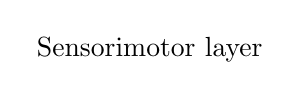
\begin{tikzpicture}
        \node at (0,0) (sensori) {Sensorimotor layer};
        %\node [subpart, below=0.2 of sensori.south west, anchor=north west, align=left] (perception) {{\bf Perception} \\ 2D markers, RGB-D, motion capture};
        %\node [subpart, align=right, right=0.2 of perception] {{\bf Actuation} \\ Head's pan-tilt unit, grippers, arms, wheels};
      \end{tikzpicture}
  };
  }

  %%% Separation between deliberative layer and sensori-motor layer
  \draw[dotted, thick] (-8,-5.5) -- (12, -5.5);

  %%% Relations between components
  \path (shary.340) edge [<->, bend left] (mhp);
  \path (shary.west) edge [<->, bend right] (hatp);
  \path (hatp) edge [<->, bend right] (oro.170);
  \path (dialogs) edge [<->, bend left] (oro.190);
  \path (spark.100) edge [->, bend right] (oro);
  \path (spark.5) edge [->, bend right] (mhp);
  \path (shary) edge [<->, bend left] (oro);
  \path (shary) edge [<->, bend left] (spark);
  \path (lowlevel) edge [->] (spark);
  \only<2,6>{
  \path (lowlevel1) edge [->] (spark);
  \path (lowlevel2) edge [->] (spark);
  }
  \path (lowlevel.east) edge [<-, bend right=80, looseness=1.5] (shary.east);

\end{tikzpicture}
}
}


\end{frame}

\begin{frame}{Hybrid architectures: epistemic arguments}

    The {\bf computational functionalism} argument~\cite{vernon2014artifical}:
    \begin{quote}
        \doublequoted{the physical realization of the computational model is inconsequential to the model}
    \end{quote}

    \uncover<2>{
        Embodied cognition takes the opposite view.\par
        
        Some see the symbolic/sub-symbolic questions as an instantiation of this argument.
    }

\end{frame}

\begin{frame}{Cross-disciplinary ``Impedance Matching''}

    The choice of a computational model impacts how {\bf legible} the architecture is
    to other disciplines:

    \begin{itemize}
        \item {\bf psycholinguistics} will be more comfortable manipulating
            symbolic architectures;
        \item {\bf neurosciences} may be more comfortable with certain
            sub-symbolic approaches (but not all of them: deep learning 
            is hardly a biologically inspired neural technique)
    \end{itemize}
    
    {\bf $\Rightarrow$ ``epistemic impedance''}

    \only<2>{
        Some disciplines are however mostly {\bf agnostic}\\
        cognitive psy., developmental psy.,...
    }

    \only<3>{
        Also relevant is the nature of {\bf predictions} you want to
        generate or test (eg, reaction time vs language competencies).
    }


\end{frame}

\begin{frame}{A few internal cognitive functions}

    \begin{table}[]
        \begin{tabularx}{\linewidth}{lp{4.5cm}p{4.5cm}}
            \toprule
                     & {\bf Symbolic}  & {\bf Sub-symbolic}\\
            \midrule
            {\bf Concepts} & taxonomies, \newline external knowledge integration & conceptualization \\
            {\bf Memory}   & facts storage & associative memory,\newline priming \\
            {\bf Planning}   & Plenty\newline (prototypically: HTN) & recurrent
            networks~\cite{rueckert2016recurrent} \\
            ... & & \\
            \bottomrule
        \end{tabularx}
        \label{tab:options}
    \end{table}
\end{frame}

\begin{frame}{Side-to-side}

    \scriptsize
    \begin{multicols}{2}

        \centering{\bf Symbolic}

    \begin{itemize}
        \item {\bf well-established theoretical grounds} in formal logics
        \item {\bf explicit}, {\bf high-level semantics}
        \item good engineering properties (modular, loose coupling,...)
        \item $\Rightarrow$ {\bf close to the human level} (both for the users and the developers)
        \item {\bf very successful} so far
        \item {\bf fundamentally top-down} approach $\Rightarrow$ somewhat difficult to match with
            the constructive approach of developmental psychology
        \item {\bf learning} is an {\bf after-thought}
        \item representation of {\bf uncertainty not natural}
        \item {\bf hard to deal with time} (chronicles, fluents,...?)
    \end{itemize}

    \columnbreak

    \centering{\bf Sub-symbolic}

    \begin{itemize}
        \item often {\bf principled approaches}
        \item {\bf learning} is intrinsic and fundamental
        \item {\bf interesting features} come for free (eg concept priming)
        \item principled approach brings {\bf predictive power}
        \item applications to high-level socio-cognitive tasks only emerging
        \item {\bf still hard to deal with time!}
    \end{itemize}

    \end{multicols}
\end{frame}


\begin{frame}{Bibliography}
\begin{thebibliography}{10}
\footnotesize
    \beamertemplatearticlebibitems
    \bibitem{baxter2013cognitive}
    P. Baxter, J. de Greeff, T. Belpaeme
    \newblock \doublequoted{Cognitive Architecture for HRI: Towards behavioural
    alignment}
    \newblock 2013


    \beamertemplatearticlebibitems
    \bibitem{lemaignan2012towards}
    S. Lemaignan, R. Alami, A. K. Pandey, M. Warnier, J. Guitton
    \newblock \doublequoted{Towards Grounding Human-Robot Interaction}
    \newblock 2012

    \beamertemplatearticlebibitems
    \bibitem{morse2010epigenetic}
    A. Morse, J. de Greeff, T. Belpaeme, A. Cangelosi
    \newblock \doublequoted{Epigenetic Robotics Architecture}
    \newblock 2010

    \beamertemplatearticlebibitems
    \bibitem{rueckert2016recurrent}
    A. Rueckert, D. Kappel, D. Tanneberg, D. Pecevski, J. Peters
    \newblock \doublequoted{Recurrent Spiking Networks Solve Planning Tasks}
    \newblock 2016


    \beamertemplatebookbibitems
    \bibitem{vernon2014artifical}
    D. Vernon
    \newblock \doublequoted{Artificial Cognitive Systems}
    \newblock 2013


  \end{thebibliography}
\end{frame}


\end{document}
